\chapter{背景}  
\label{chapter:introduction}  

在当今全球科技飞速发展的背景下,科技创新已成为推动社会进步与国家发展的核心动力。正如习近平总书记所指出的:“科技创新是发展新质生产力的核心要素。”科技创新不仅为经济增长注入活力,更为提升国家综合竞争力奠定了坚实基础。

根据国家统计局发布的报告,创新指数体系涵盖四大类与二十个小类指标,全面覆盖创新活动的各个维度(见表\ref{创新指数构成表_上}和表\ref{创新指数构成表_下})。该指标体系为深入分析国家创新能力提供了科学依据,同时也为我们评估科技前沿动态提供了可靠的数据支撑。

\begin{table}[H]
\centering
\caption{创新指数构成表(上)}
\begin{tabular}{lll}
\toprule
\textbf{分领域} & \textbf{指标名称} & \textbf{占比} \\
\midrule
\multirow{5}{*}{创新环境(1/4)} 
    & 1.1 每万人就业人员中大专及以上学历人数 & 1/5 \\
    & 1.2 人均GDP & 1/5 \\
    & 1.3 理工类毕业生占适龄人口比重 & 1/5 \\
    & 1.4 科技拨款占财政拨款比重 & 1/5 \\
    & 1.5 享受加计扣除减免税企业所占比重 & 1/5 \\
\midrule
\multirow{4}{*}{创新投入(1/4)} 
    & 2.1 每万人R\&D人员全时当量 & 1/4 \\
    & 2.2 R\&D经费占GDP比重 & 1/4 \\
    & 2.3 基础研究人员人均经费 & 1/4 \\
    & 2.4 企业R\&D经费占营业收入比重 & 1/4 \\
\midrule
\multirow{4}{*}{创新产出(1/4)} 
    & 3.1 每万人科技论文数 & 1/4 \\
    & 3.2 每万名R\&D人员高价值发明专利拥有量 & 1/4 \\
    & 3.3 拥有注册商标企业所占比重 & 1/4 \\
    & 3.4 技术市场成交合同平均金额 & 1/4 \\
\bottomrule
\label{创新指数构成表_上}
\end{tabular}
\end{table}

\begin{table}[H]
\centering
\caption{创新指数构成表(下)}
\begin{tabular}{lll}
\toprule
\textbf{分领域} & \textbf{指标名称} & \textbf{占比} \\
\midrule
\multirow{5}{*}{创新成效(1/4)} 
    & 4.1 新产品销售收入占营业收入比重 & 1/5 \\
    & 4.2 高新技术产品出口额占货物出口额比重 & 1/5 \\
    & 4.3 专利密集型产业增加值占GDP比重 & 1/5 \\
    & 4.4 “三新”经济增加值占GDP比重 & 1/5 \\
    & 4.5 全员劳动生产率 & 1/5 \\
\bottomrule
\label{创新指数构成表_下}
\end{tabular}
\end{table}

党的十四届全国人大三次会议审议通过了一系列旨在推动科技创新、促进产业升级和深化社会改革的重要政策,充分彰显了战略转型的坚定决心。特别是在政府工作报告中提出的“人工智能+”行动计划,标志着我国在人工智能领域的战略部署迈入新阶段。

此外,会议还强调,社会改革应与科技进步协同推进,尤其是在教育体系改革与人才培养机制建设方面。随着人工智能、机器人、大数据等前沿技术不断取得突破,传统就业结构与职业模式正经历深刻变化。大会明确提出,要加快教育改革步伐,着力培养符合新时代要求的复合型人才,这既是应对产业结构变迁与劳动力市场调整的必要之举,也是实现社会可持续发展的根本保障。

在深入贯彻创新驱动发展战略的背景下,本文将围绕教育、企业、就业及国际竞争力等关键领域,基于国家政策导向与科技发展趋势展开多角度分析\cite{chen2021beyond}。为明确研究方向,本文通过词云技术对政策文本进行可视化处理,为下文研究提供了理论依据与分析线索(见图\ref{fig:词云})。

\begin{figure}[H]
    \centering
    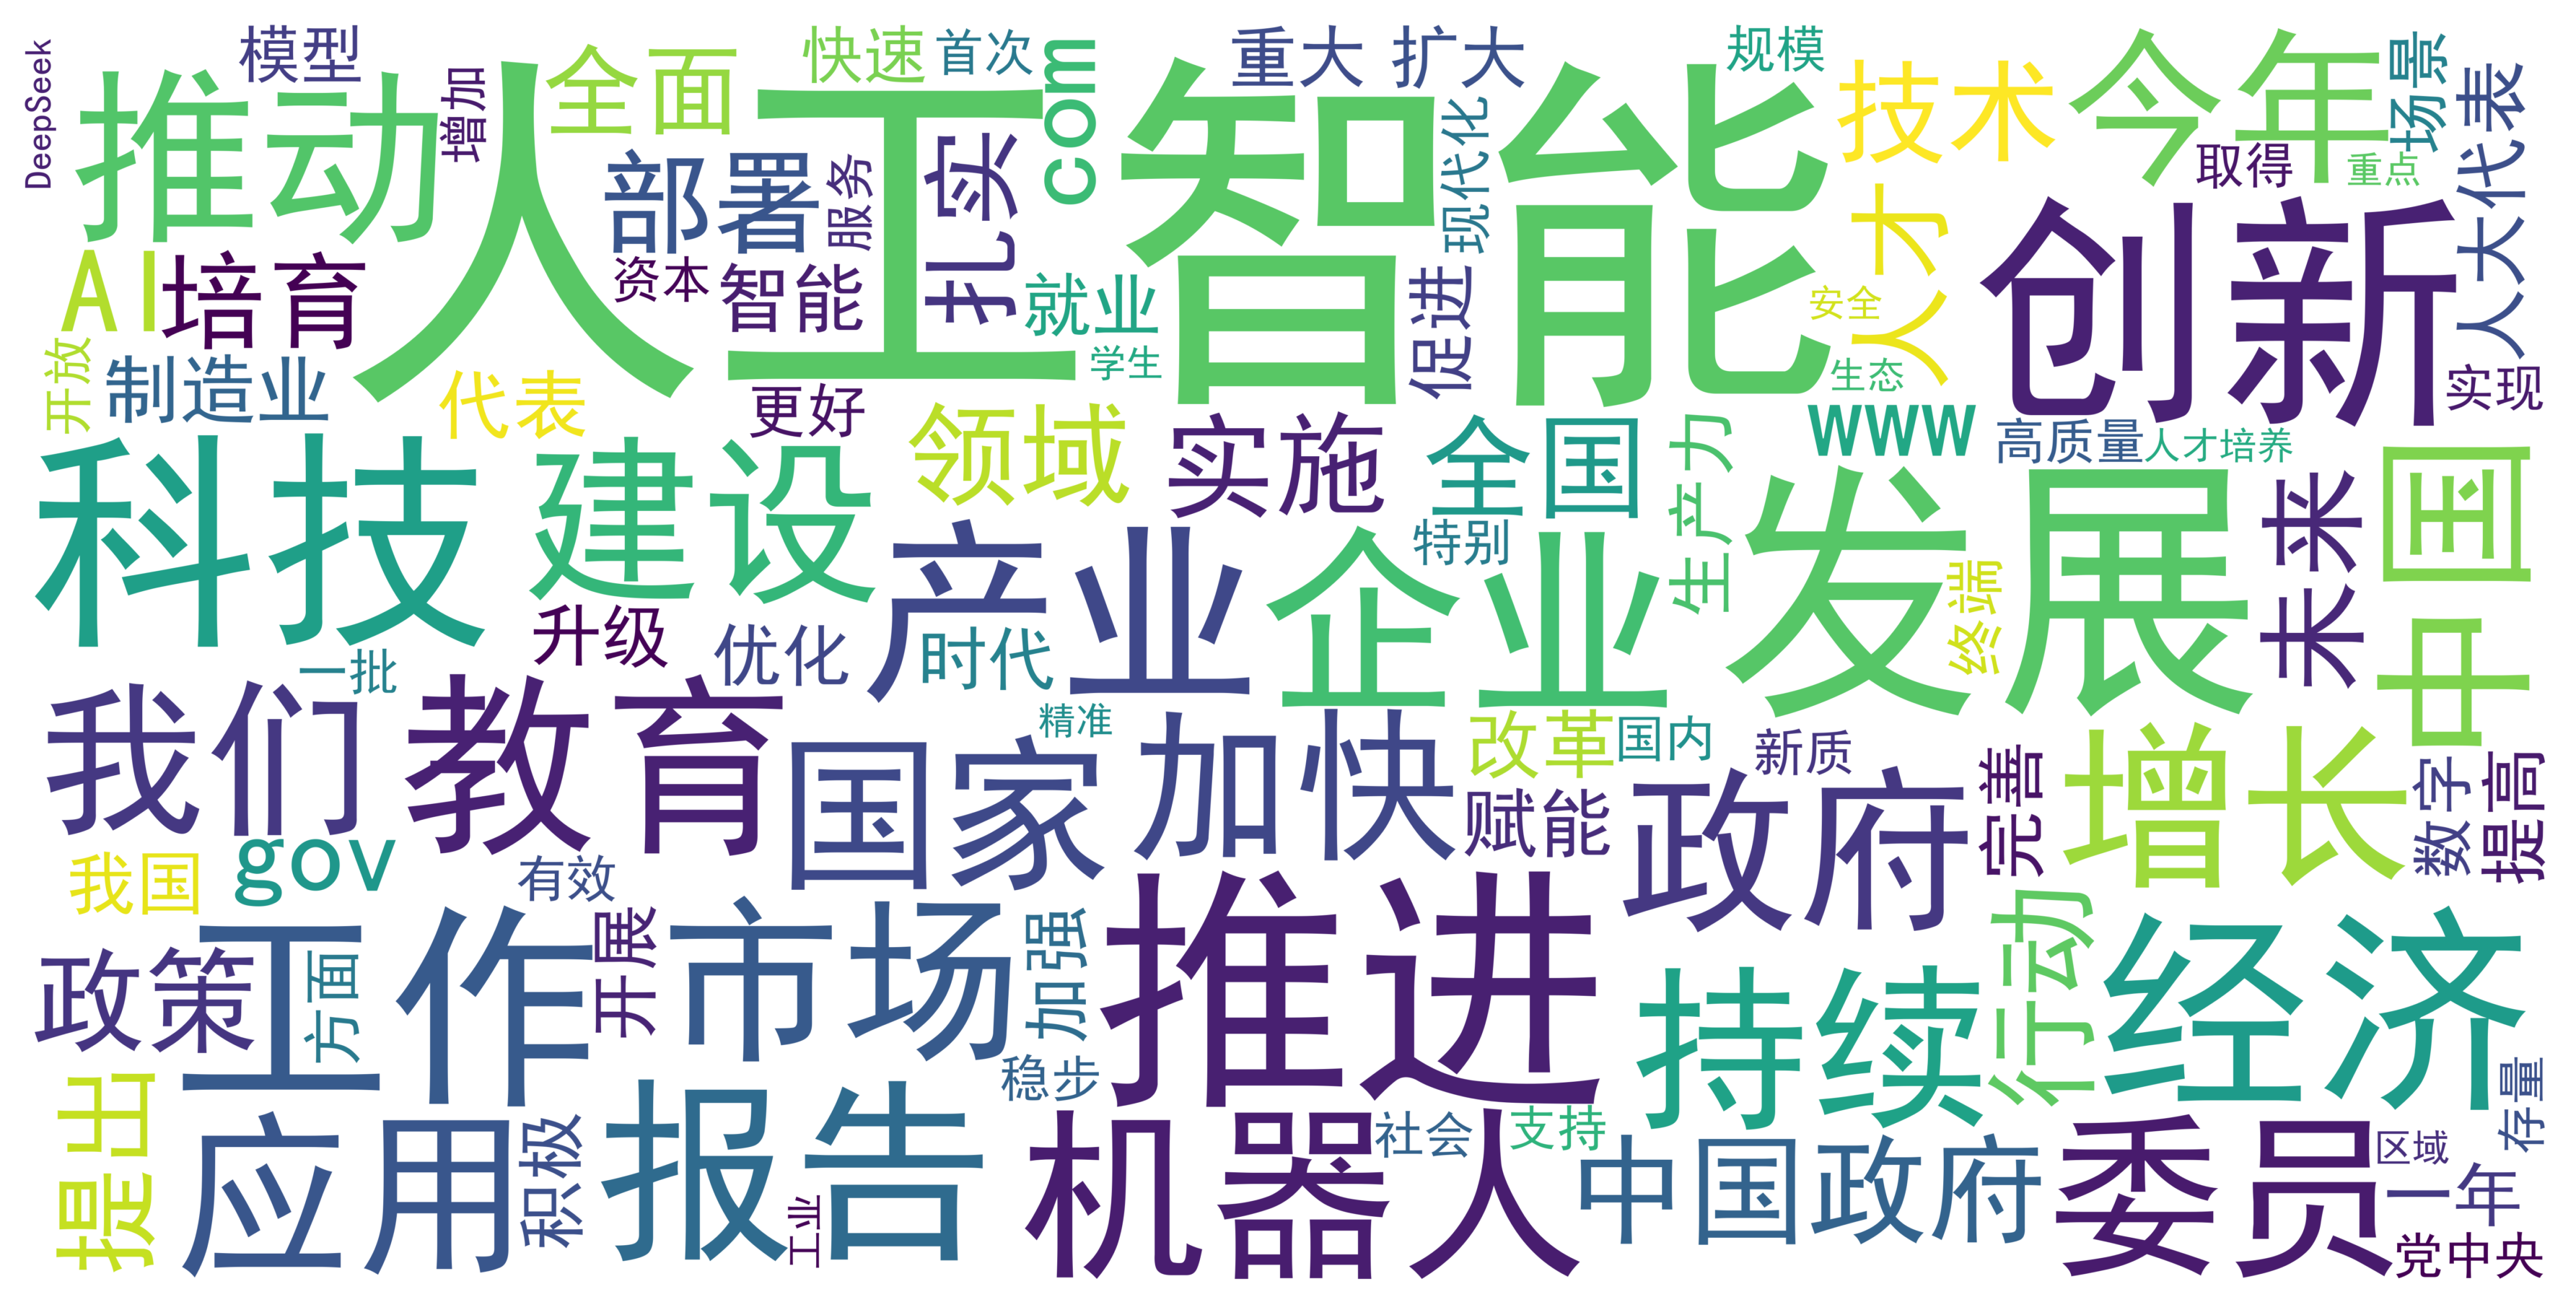
\includegraphics[width=0.5\linewidth]{figure/wordcloud_output.png}
    \caption{政策关键词词云图}
    \label{fig:词云}
\end{figure}

从词云图中可以看出,国家政策密切聚焦于教育体系优化、企业创新能力建设、人才结构转型与国际竞争力提升等核心议题。不仅反映了当前社会关注的重点方向,也为后续章节的深入探讨提供了清晰的研究主线,力求揭示国家政策与科技发展之间的互动机制,以及其在推动社会变革中的深层作用。

